\documentclass{report}

\input{~/dev/latex/template/preamble.tex}
\input{~/dev/latex/template/macros.tex}

\title{\Huge{Methods Of Integration Pre Calc 2}}
\author{\huge{Nathan Warner}}
\date{\huge{}}
\pagestyle{fancy}
\fancyhf{}
\lhead{Warner \thepage}
\rhead{}
% \lhead{\leftmark}
\cfoot{\thepage}
\setborder
% \usepackage[default]{sourcecodepro}
% \usepackage[T1]{fontenc}

\begin{document}
    % \maketitle
    \begin{titlepage}
       \begin{center}
           \vspace*{1cm}
    
           \textbf{Methods Of Integration}
    
           \vspace{0.5cm}
            Pre Calculus 2
                
           \vspace{1.5cm}
    
           \textbf{Nathan Warner}
    
           \vfill
                
                
           \vspace{0.8cm}
         
           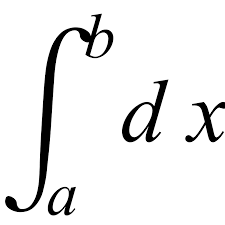
\includegraphics[width=0.4\textwidth]{./figures/int.png}
                
           Mathematics \\
           Northern Illinois University\\
           United States\\
           May 26,2023
                
       \end{center}
    \end{titlepage}
    
    \tableofcontents
    \pagebreak \bigbreak \noindent
    \bigbreak \noindent 
    \section{\Large{U-Substitution}}
          \bigbreak \noindent \bigbreak \noindent
      If $u=g(x)$ is differentiable and its range $\in I $ and $f $ is continuous on $I$, then
      \begin{align*}
        \int f(g(x))g^{\prime}(x)\ dx = \int f(u)\ du
      .\end{align*}
      \bigbreak \noindent \bigbreak \noindent
      \textbf{\textit{\underline{Process:}}}
      \begin{enumerate}
        \item Make a decent choice of what to let u equal
        \item Change our integral from being in terms of $x$, to in terms of $u$
        \item Integrate $\int f(u)\ du $
        \item Change back to $x$
      \end{enumerate}
      \bigbreak \noindent \bigbreak \noindent
      \nt{Also include the constant in your u sub, if it is attached to the function you let u equal,
        Also note for rational trig functions, you can move trig functions from upstairs or downstairs based on their reciprical function, for example, a $\cos^{2}{x}$ in the denominator can be
        moved upstairs as $\sec^{2}{x}$
      }
      \bigbreak \noindent \bigbreak \noindent
      \textbf{\textit{\underline{Notes:}}}
      \begin{itemize}
       \item Our goal with u-sub is to let u equal some function in our composition of functions, such that if we derive that function, we get back something that is also in our integrand
        \item Say we have something like:
          \begin{align*}
            \int \sec^{2}{\theta }\ d\theta  \\ 
            Let\ u = 8\theta  \\
            du = 8d\theta  \\
            \frac{1}{8}du = d\theta 
          .\end{align*}
        \item Know that you can rewrite equations like:
          \begin{align*}
            \int \frac{(\ln{x})^{36}}{x}\ dx \\
            as: \int \frac{1}{x}(\ln{x})^{36}\ dx
          .\end{align*}
        \item Say we have:
          \begin{align*}
            -\frac{1}{2} \int_{0}^{-1}\ e^{u}\ du
          .\end{align*}
          \begin{itemize}
            \item We can flip the limits of integration to remove the negative sign. So we will have:
          \end{itemize}
            \begin{align*}
              \frac{1}{2}\int_{-1}^{0}\ e^{u}\ du
            .\end{align*}
          \item Look out for being able to turn antiderivative into inverse trig functions.
            \begin{itemize}
              \item Say we have:
            \begin{align*}
              \int \frac{x^{7}}{1+x^{16}}\ dx
            .\end{align*}
          \item Don't let $u=1+x^{8} $, we could do this by turning $x^{16}\ into\ (x^{8})^{2}$, but instead, just let $u=x^{8}$. We do this because it ends up like:
            \begin{align*}
             \frac{1}{8}du = x^{7}dx  
            .\end{align*}
          \item So when we sub we get that nice arctan antiderivative, just something to look out for.
            \begin{align*}
              \frac{1}{8}\int \frac{1}{1+u^{2}}\ du
            .\end{align*}
            \end{itemize}
          \item Note that we can write:
            \begin{align*}
              e^{2x}
            .\end{align*}
            \begin{itemize}
              \item as 
            \end{itemize}
            \begin{align*}
              (e^{x})^{2}
            .\end{align*}
      \end{itemize}

      \bigbreak \noindent \bigbreak \noindent
       \textbf{\textit{\underline{Definite Integrals with u-sub}}} 
      \begin{enumerate}
        \item Find what u is going to equal
        \item Find u(a) and u(b) 
        \item make u-sub and use u(a) and u(b) as limits of integration
        \item find antiderivative and evaluate at new limits
      \end{enumerate}
      \bigbreak \noindent 
      \nt{For definite integrals, don't sub back in for u, just evalute integral with u still subbed}

      \pagebreak \bigbreak \noindent
      \section{Integrals of Symmetric functions.}
      \bigbreak \noindent \bigbreak \noindent
      \textbf{Sometimes you will run into integrals that are either impossible, or too difficult with u Substitution. For these cases we will look at Integrals of Symmetric Functions}
      \bigbreak \noindent \bigbreak \noindent
      \textbf{\textit{\underline{Even:}}} 
      \begin{align*}
        f(-x)  = f(x)\ then\ \int_{-a}^{a}\ f(x)\ dx  = 2 \int_{0}^{a}\ f(x)\ dx
      .\end{align*}
      \bigbreak \noindent \bigbreak \noindent
      \textbf{\textit{\underline{Odd:}}}
      \begin{align*}
        f(-x) = -f(x)\ then\ \int_{-a}^{a}\ f(x)\ dx = 0
      .\end{align*}

      \bigbreak \noindent \bigbreak \noindent
      \textbf{\textit{\underline{Notes:}}}
      \begin{itemize}
        \item If a function is even, you can replace your lower limit with zero and multiply the integral by 2
        \item if a function is odd, then the integral equals zero.
      \end{itemize}

      \bigbreak \noindent \bigbreak \noindent
      \textbf{\textit{\underline{Figures:}}}
      \begin{figure}[ht]
          \centering
          \incfig{fig1even}
          \incfig{fig2even}
          \label{fig:fig1even}
      \end{figure}

      \pagebreak \bigbreak \noindent
      \section{\Large{Integration By Long Division.}}
      \bigbreak \noindent 
      Long division is typically used when evaluating integrals that involve rational functions, where the numerator's degree is equal to or greater than the denominator's degree. By performing long division, you can rewrite the rational function as a sum of a polynomial and a proper rational function, making it easier to integrate.
      \bigbreak \noindent 
      Consider the integral
      \begin{align*}
          \int \frac{x-5}{-2x+2}\ dx
      .\end{align*}
      \bigbreak \noindent 
      So with long division, we have:
      \begin{align*}
          -2x+2 \overline{)x-5}
      .\end{align*}
      \bigbreak \noindent \bigbreak \noindent 
      We get $-\frac{1}{2}$, with a remainder of $-4$, which would be $\frac{4}{-2x+2} $. So now our integral would be:
      \bigbreak \noindent 
      \begin{align*}
          \int \bigg(-\frac{1}{2} - \frac{4}{-2x+2}\bigg)\ dx \\
          = \int \bigg(-\frac{1}{2} - \frac{2}{-x+1}\bigg)\ dx \\
          = \int \bigg(-\frac{1}{2} - \bigg(-\frac{2}{x-1}\bigg)\bigg)\ dx \\
          = \int \bigg(-\frac{1}{2} + \frac{2}{x-1}\bigg)\ dx
      .\end{align*}
      \bigbreak \noindent 
      Now we can split up our integral:
      \begin{align*}
          \int -\frac{1}{2}\ dx + \int \frac{2}{x-1}\ dx
      .\end{align*}
      \bigbreak \noindent 
      We can see that our first integral will evaluate to $-\frac{1}{2}x + C $, and we can use U-Sub for the second integral:
      \begin{align*}
          \int \frac{2}{x-1}\ dx \\
          = \int \frac{1}{x-1}2\ dx \\
          = 2\int \frac{1}{x-1}\ dx \\
          \text{Let $u=x-1$} \\
          du = dx \\
        = 2\int \frac{1}{u}\ du = 2\int u^{-1}\ dx \\
        = 2\ln{\abs{u}} + C \\
        = 2\ln{\abs{x-1} + C}
      .\end{align*}
      \bigbreak \noindent \bigbreak \noindent 
      So our full solution is:
      \begin{align*}
          -\frac{1}{2}x + 2\ln{\abs{x-1} + C}
      .\end{align*}

      \pagebreak \bigbreak \noindent
      \section{Integration By Completing The Square.}
      \bigbreak \noindent 
      Completing the square is a technique commonly used in algebra to rewrite quadratic expressions. While it is not typically used directly for evaluating integrals, completing the square can be helpful in certain situations when dealing with quadratic forms within integrals. Here are two scenarios where completing the square can be useful for evaluating integrals:

      \begin{itemize}
          \item Quadratic Denominators: When you encounter an integral with a quadratic denominator, completing the square can help in simplifying the expression. By completing the square, you can rewrite the quadratic expression in a form that allows for a straightforward integration.
      \end{itemize}

      \bigbreak \noindent 
      Consider the integral:
      \begin{align*}
          \int \frac{1}{5x^{2} -30x+65}\ dx
      .\end{align*}
      \bigbreak \noindent \bigbreak \noindent 
      We can first start by factoring out a 5 from the denominator and moving it outside the integral.
      \begin{align*}
          \int \frac{1}{5(x^{2} - 6x +13)}\ dx \\
          = \frac{1}{5} \int \frac{1}{x^{2} - 6x + 13}\ dx
      .\end{align*}
      \bigbreak \noindent \bigbreak \noindent 
      Now we can complete the square.
      \begin{align*}
          \frac{1}{5} \int \frac{1}{x^{2}-6x + \bigg(\frac{-6}{2}\bigg)^{2} - \bigg(\frac{-6}{2}\bigg)^{2} +13}\ dx \\
           = \frac{1}{5}\int \frac{1}{x^{2}-6x + 9 - 9 + 13}\ dx \\
           = \frac{1}{5} \int \frac{1}{(x-3)^{2} + 2^{2}}\ dx
      .\end{align*}
      \bigbreak \noindent 
      \nt{We also subtracted 9 from the denominator as to not break any rules.}
      \bigbreak \noindent \bigbreak \noindent 
      Now our goal is to make this $\arctan{}$, so we are going to divide everything by $2^{2}$ to get that +1 in the denominator.
      \bigbreak \noindent 
      So we get:
      \begin{align*}
          \frac{\frac{1}{5}}{4}\cdot \int \frac{\frac{1}{2^{2}}}{\frac{(x-3)^{2}}{2^{2}} + \frac{2^{2}}{2^{2}}}\ dx \\
          \frac{1}{20}\int \frac{1}{\bigg(\frac{(x-3)}{2}\bigg)^{2} + 1}\ dx
      .\end{align*}
      \bigbreak \noindent \bigbreak \noindent 
      Now we can use U-Sub to evalute this integral:
      \begin{align*}
          \text{Let}\ u=\frac{1}{2}x - \frac{3}{2} \\
          du = \frac{1}{2}dx \\
          2du = dx
      .\end{align*}
      \bigbreak \noindent \bigbreak \noindent 
      So we have:
      \begin{align*}
          2 \cdot \frac{1}{20} \int \arctan{u}\ du \\
          = \frac{1}{10}\arctan{u}  + C \\
          = \frac{1}{10} \arctan{\bigg(\frac{x-3}{2}}\bigg)  + C 
      .\end{align*}

      \bigbreak \noindent \bigbreak \noindent 
      \ex{Evalute the integral by completing the square}{
          \begin{align*}
              \int \frac{1}{\sqrt{-x^{2}-6x+40}}\ dx
          .\end{align*}
          \bigbreak \noindent 
          By the looks of it, our goal will be to turn this into arcsine. So our first step will be to write the radical as:
          \begin{align*}
              \int \frac{1}{\sqrt{40-x^{2}-6x)}}\ dx
          .\end{align*}
          \bigbreak \noindent 
          Because our goal is for this to resemble:
          \begin{align*}
              \frac{d}{dx}\sin^{-1}{x} \\
              = \frac{1}{\sqrt{1-x^{2}}}
          .\end{align*}
          \bigbreak \noindent 
          Now if we complete square:
          \begin{align*}
              \int \frac{1}{\sqrt{40 -x^{2}-6x+\bigg(\frac{-6}{2}\bigg)^{2} -\bigg(-\frac{6}{2}\bigg)^{2} }}\ dx \\
              = \int \frac{1}{\sqrt{40 - x^{2} - 6x + 9 -9}}\ dx \\
              = \int \frac{1}{\sqrt{40 + 9 - x^{2} - 6x -9}}\ dx \\
              = \int \frac{1}{\sqrt{-(-40 - 9 + x^{2} + 6x +9)}}\ dx \\
              = \int \frac{1}{\sqrt{-(-49 +(x+3)^{2})}}\ dx \\
              = \int \frac{1}{\sqrt{49 -(x+3)^{2})}}\ dx \\
              = \int \frac{1}{\sqrt{7^{2} -(x+3)^{2})}}\ dx \\
          .\end{align*}
          \bigbreak \noindent 
          Now if we let $u=x+3$, then $du= dx$, so we have:
          \begin{align*}
              \int \frac{1}{\sqrt{7^{2}-u^{2}}}\ du \\
              = \int \frac{1}{\sqrt{\frac{7^{2}}{7^{2}}- \frac{u^{2}}{7^{2}}}}\ du \\
              = \int \frac{1}{\sqrt{1-\bigg(\frac{u}{7}\bigg)^{2}}}\ du 
          .\end{align*}
          \bigbreak \noindent 
          Which we can evaluate as:
          \begin{align*}
              \arcsin{\bigg(\frac{u}{7}\bigg) + C} \\
              \boxed{=\arcsin{\bigg(\frac{x+3}{7}\bigg)} + C }
          .\end{align*}
      }
      \bigbreak \noindent 
      \ex{}{
          Problem:
          \begin{align*}
              \int \frac{1}{(x-7)^{2} + 3^{2}}\ dx
          .\end{align*}
          \bigbreak \noindent 
          Accepted Answer:
          \begin{align*}
              \frac{1}{3}\arctan{\bigg(\frac{x-7}{3}\bigg) + C}
          .\end{align*}
          \bigbreak \noindent 
          My Work
          \begin{align*}
              1\cdot \int \frac{1}{(x-7)^{2} + 3^{2}}\ dx \\
              = \frac{1}{3^{2}} \int \frac{1}{\bigg(\frac{(x-7)}{3}\bigg)^{2} + \frac{3^{2}}{3^{2}}}\ dx \\
              = \frac{1}{9} \int \frac{1}{\bigg(\frac{(x-7)}{3}\bigg)^{2} + 1}\ dx \\
          .\end{align*}
          \begin{align*}
              Let\ u= \frac{1}{3}x - \frac{7}{3} \\
              du = \frac{1}{3}dx \\
              3du = dx
          .\end{align*}
          \begin{align*}
              3 \cdot \frac{1}{9} \int \frac{1}{u^{2} + 1}\ dx \\
              = \frac{1}{3}\tan^{-1}{u} + C \\
              = \frac{1}{3}\tan^{-1}{\bigg(\frac{x-7}{3}\bigg) + C}
          .\end{align*}
      }





    
\end{document}
